\documentclass[11pt]{article}
\usepackage{geometry}                % See geometry.pdf to learn the layout options. There are lots.
\geometry{a4paper}                   % ... or a4paper or a5paper or ... 
\usepackage{graphicx}
\usepackage{amssymb}
\usepackage{url}
\usepackage{listings}
\usepackage{color}

\renewcommand{\textfraction}{0.15}
\renewcommand{\topfraction}{0.85}
\renewcommand{\bottomfraction}{0.65}
\renewcommand{\floatpagefraction}{0.60}

\lstset{ %
language=C++,                  %choose the language of the code
basicstyle=\footnotesize\ttfamily,% the size of the fonts that are used for the code
showstringspaces=false,         % underline spaces within strings
numbers=left,                   % where to put the line-numbers
numberstyle=\ttfamily,      % the size of the fonts that are used for the line-numbers
stepnumber=2,                   % the step between two line-numbers. If it's 1 each line will be numbered
numbersep=5pt,                  % how far the line-numbers are from the code
stringstyle=\ttfamily,          % typewriter type for strings
backgroundcolor=\color{white},  % choose the background color
showspaces=false,               % show spaces within strings adding particular underscores
showtabs=false,                 % show tabs within strings adding particular underscores
escapeinside={\%*}{*)},         % if you want to add a comment within your code
breaklines=true,                 % break line if it is too long
frame=leftline
}

\usepackage{fontspec,xltxtra,xunicode}
\defaultfontfeatures{Mapping=tex-text}
\setromanfont[Mapping=tex-text]{Georgia}
\setsansfont[Scale=MatchLowercase,Mapping=tex-text]{Tahoma}
\setmonofont[Scale=MatchLowercase]{Courier New}


\title{IEG4180 Project 1\\NetProbe Documentation}
\author{GUAN Hao\\05569511\\hguan5@ie.cuhk.edu.hk}
\date{\today}
\begin{document}
\maketitle
\section{Introduction}
The {\em NetProbe} is a simple network program which is implemented on Microsoft Visual C++ with winsock API. It has 2 primary features: Host Information and Send/Receive Test.

In {\em Host Information} Mode, the program can be used to resolve domain name or IP address and show the official name of the host and a list of return IP addresses.

In Send/Receive Test Mode, either TCP or UDP protocol can be chosen. User can also specify the {\em Sending Rating, Refresh Rate, Packet Size} and {\em Number of Packets to send}. Transmission statistics will be displayed and updated according to the specified refresh rate.
\section{Program Structure}
The program is a MFC application which is designed with the Object-Oriented concept. Following is the list of classes implemented in this program:
\begin{itemize}
\item {\tt class CNetProbeApp}, the main class of this program. This class will create a instance of {\tt class CNetProbeDlg} and show the dialog. Some {\tt winsock} initialize functions are also invoked here.
\item {\tt class CNetProbeDlg}, this class control the main dialog of the application. 
\item {\tt class NetProbe}, all the socket operation is implemented in this class. Following shows the prototype of {\tt class NetProbe}:
\begin{lstlisting}
class NetProbe{
public:
	NetProbe();
	BOOL startSend();
	BOOL startReceive();
	void stop(void);
	void stop(BOOL n);
	void setLocal(char *h);
	void setRemote(char *h);
	void setLocalPort(int n);
	void setRemotePort(int n);
	void setRefreshInterval(int t);
	void setPacketSize(int n);
	void setSendingRate(int n);
	void setNumPackets(int n);
	void setProtocol(int p);
	void setStatus(int n);
	int getMaxNum(void);
	int getPacketTransfer(void);
	int getTransferRate(void);
	double getPacketLoss(void);
	int getPacketLost(void);
	double getTime(void);
	int getStatus(void);
	char *getLocal(void);
	char *getRemote(void);
	int getLocalPort(void);
	int getRemotePort(void);
	int getPacketSize(void);
	int getInterval(void);
	int getNumPackets(void);
	double getByteTransfer(void);
	void packetTransfer(int n);
	void byteTransfer(int n);
	ES_FlashTimer timer;

private:
	int status;
	char *local;
	char *remote;
	int localPort;
	int remotePort;
	int refreshInterval;
	int packetSize;
	int sendingRate;
	int numPackets;
	int packetTransferred;
	int protocol;
	int maxPacketNum;
	double byteTransferred;
};
\end{lstlisting}
\item {\tt class CHostInfoDlg}, the Host Information function is implemented in this class. When {\em HostInfo} button on the main dialog is clicked, this dialog will appear. 
\end{itemize}
\section{GUI Design}
\begin{figure}
\centering
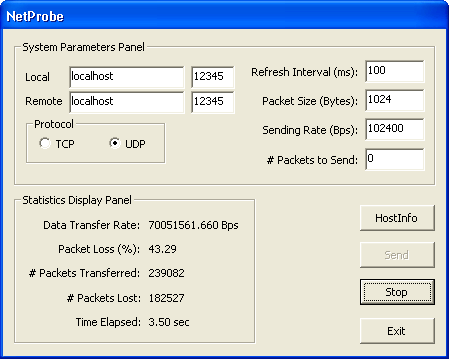
\includegraphics[width=3in]{work.png}
\caption{Statistics shown on the dialog.}
\label{fig:work}
\end{figure}
The main dialog is designed as in Figure \ref{fig:work}. User can input parameters and choose protocol on this dialog.After {\em Send} or {\em Receive} button is clicked, the caption of the button will turn to {\em Stop}. During transmission, the statistics will be shown on the bottom of the dialog.

\begin{figure}
\centering
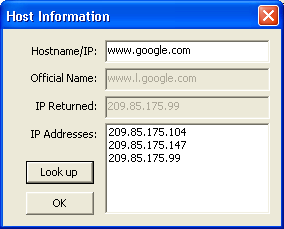
\includegraphics[width=3in]{hostinfo.png}
\caption{Host Information Dialog.}
\label{fig:hostinfo}
\end{figure}
The Host Information is designed very easy to use. Just input the domain name or IP address in the edit box and click the {\em Look Up} button the result will show(See Figure \ref{fig:hostinfo}) or if the domain name cannot not be resolved, a message box will appear to indicate the error.



\end{document}
